%課題研究レジュメテンプレート ver. 1.2

\documentclass[uplatex]{jsarticle}
\usepackage[top=20mm,bottom=20mm,left=20mm,right=20mm]{geometry}
\usepackage[T1]{fontenc}
\usepackage{txfonts}
\usepackage{wrapfig}
\usepackage[expert,deluxe]{otf}
\usepackage[dvipdfmx,hiresbb]{graphicx}
\usepackage[dvipdfmx]{hyperref}
\usepackage{pxjahyper}
\usepackage{secdot}

\makeatletter
  \renewcommand{\section}{%
    \if@slide\clearpage\fi
    \@startsection{section}{1}{\z@}%
    {\Cvs \@plus.5\Cdp \@minus.2\Cdp}% 前アキ
    {.5\Cvs \@plus.3\Cdp}% 後アキ
    %{\normalfont\Large\headfont\raggedright}}
    {\normalfont\raggedright}}

  \renewcommand{\subsection}{\@startsection{subsection}{2}{\z@}%
    {\Cvs \@plus.5\Cdp \@minus.2\Cdp}% 前アキ
    {.5\Cvs \@plus.3\Cdp}% 後アキ
    %{\normalfont\large\headfont}}
    {\normalfont}}

  \renewcommand{\subsubsection}{\@startsection{subsubsection}{3}{\z@}%
    {\Cvs \@plus.5\Cdp \@minus.2\Cdp}%
    {\z@}%
    %{\normalfont\normalsize\headfont}}
    {\normalfont}}
\makeatother
%ここから上を編集する必要はない.





\title{\vspace{-14mm}社会実装を目的とした他学科合同プロジェクトのマネジメント}
\author{PMコース 矢吹研究室 1442069 氏名 須山 武弘}
\date{}%日付を入れる必要はない.
\pagestyle{empty}%ページ番号は振らない.
\begin{document}
\maketitle





\section{研究の背景}
少子高齢化社会の進む日本において介護業界はこれからさらに重要となっていく業界である.さらに健康寿命が短くなっており,介護の需要はさらに高いといえる.\cite{hakusyo}実際に特別養護老人ホームの入所申込者数(待機者数)は09年~14年の5年間で10万人増加している.これは,1947年~1949年に生まれた団塊世代の人たちが徐々に介護サービスを必要としてきているのが要因とも言える.\cite{minnano}

介護業界は増える要介護者に対して介護職員は賃金,労働時間,体力的,精神的な負担が多く,厳しい労働環境にあり,離職率も高い.さらに有効求人倍率が2倍を超えている状況で増える需要に介護職員の人数が追いついていないといえる.\cite{jinzai}これを解消するには介護のオートメーション化や外国人労働者の雇用,介護職員の負担軽減が必要であると考えられる.

私は介護現場を技術で支え,介護職員の負担軽減を目指す目的のもと,船橋市や南房総市多数の介護施設を見学をしてきた.

プロジェクトマネジメント学科,未来ロボティクス学科,デザイン科学科の3学科合同のチームを編成し,介護職員の負担を軽減するために使え,理想の介護であるなおかつその人らしい生活をサポートできる介護機器の開発プロジェクトを遂行した.また,この介護機器開発プロジェクトは,開発のみならず,実際に社会に売り出すことのできるところまで考える社会実装を目的とした活動である.

専門分野の異なる3学科合同で行っているため,プロジェクトマネジメント学科内だけで行っている演習とは違いそれぞれの専門分野を活かし,それぞれの意見をまとめプロジェクトを成功へ導くことが必要である.


\section{研究の目的}
開発した製品の社会実装を目的とした活動SI-LAB(Society Implementation Laboratory)で多数の介護現場を見学し,介護現場を助ける機器をプロジェクトマネジメント学科,未来ロボティクス学科,デザイン科学科の3学科の知識や特色を活かし,プロジェクトを成功へ導くことが目的である.

\section{プロジェクトマネジメントとの関連}
今回のSI-LABの活動を通してPM学科以外の他学科の特徴を踏まえたプロジェクトマネジメント及び,人的資源の適切な配分を行う.


\section{研究の方法}
2016年7月~17年2月にかけてプロジェクトマネジメント学科,未来ロボティクス学科,デザイン科学科の3学科4人チームで介護現場の問題点を発見し,それを解消するための製品開発プロジェクトを以下のように遂行する.

7月~9月 ・・・ 介護施設訪問をし,問題点を話し合い,それ補助できる製品を提案する.

9月~10月 ・・・ CVG(キャンパスベンチャーグランプリ)へ応募書類の作成.ビジネスプランの作成.

11月 ・・・ CVGの書類選考を通過.予選へ向けてのプレゼン.

12月~1月 ・・・ 実際に使える製品の製作.機構の検討.

1月~2月 ・・・ 製品の製作.介護関係者へ向けてのプレゼンの準備.

以上のスケジュールを踏まえ,3学科の特色を活かした人的資源配分をする.

\section{現在の進捗状況}

介護現場の調査へ出向き,問題点を洗い出し,メンバーでミーティングを重ねた結果,トイレ介助が介護現場の大きな負担になっている事が判明した.その点からトイレ介助の際に介護職員及び要介護者をサポートする機器を考案した.考案したプロダクトが図1である.
大学生を対象としたビジネスコンテストであるCVGに製品と合わせてビジネスプランを作成し応募した.その結果,書類選考を通過し,東京大会の予選にてプレゼンを行った.
ビジネスプランの作成及びスケジュール管理,人的資源の管理はプロジェクトマネジメント学科,プロダクトのデザインはデザイン科学科,機構及びプロダクトの強度は未来ロボティクス学科が担当し,それぞれの専門分野を活かした活動ができている.

\begin{figure}[htbp]
  \begin{center}
    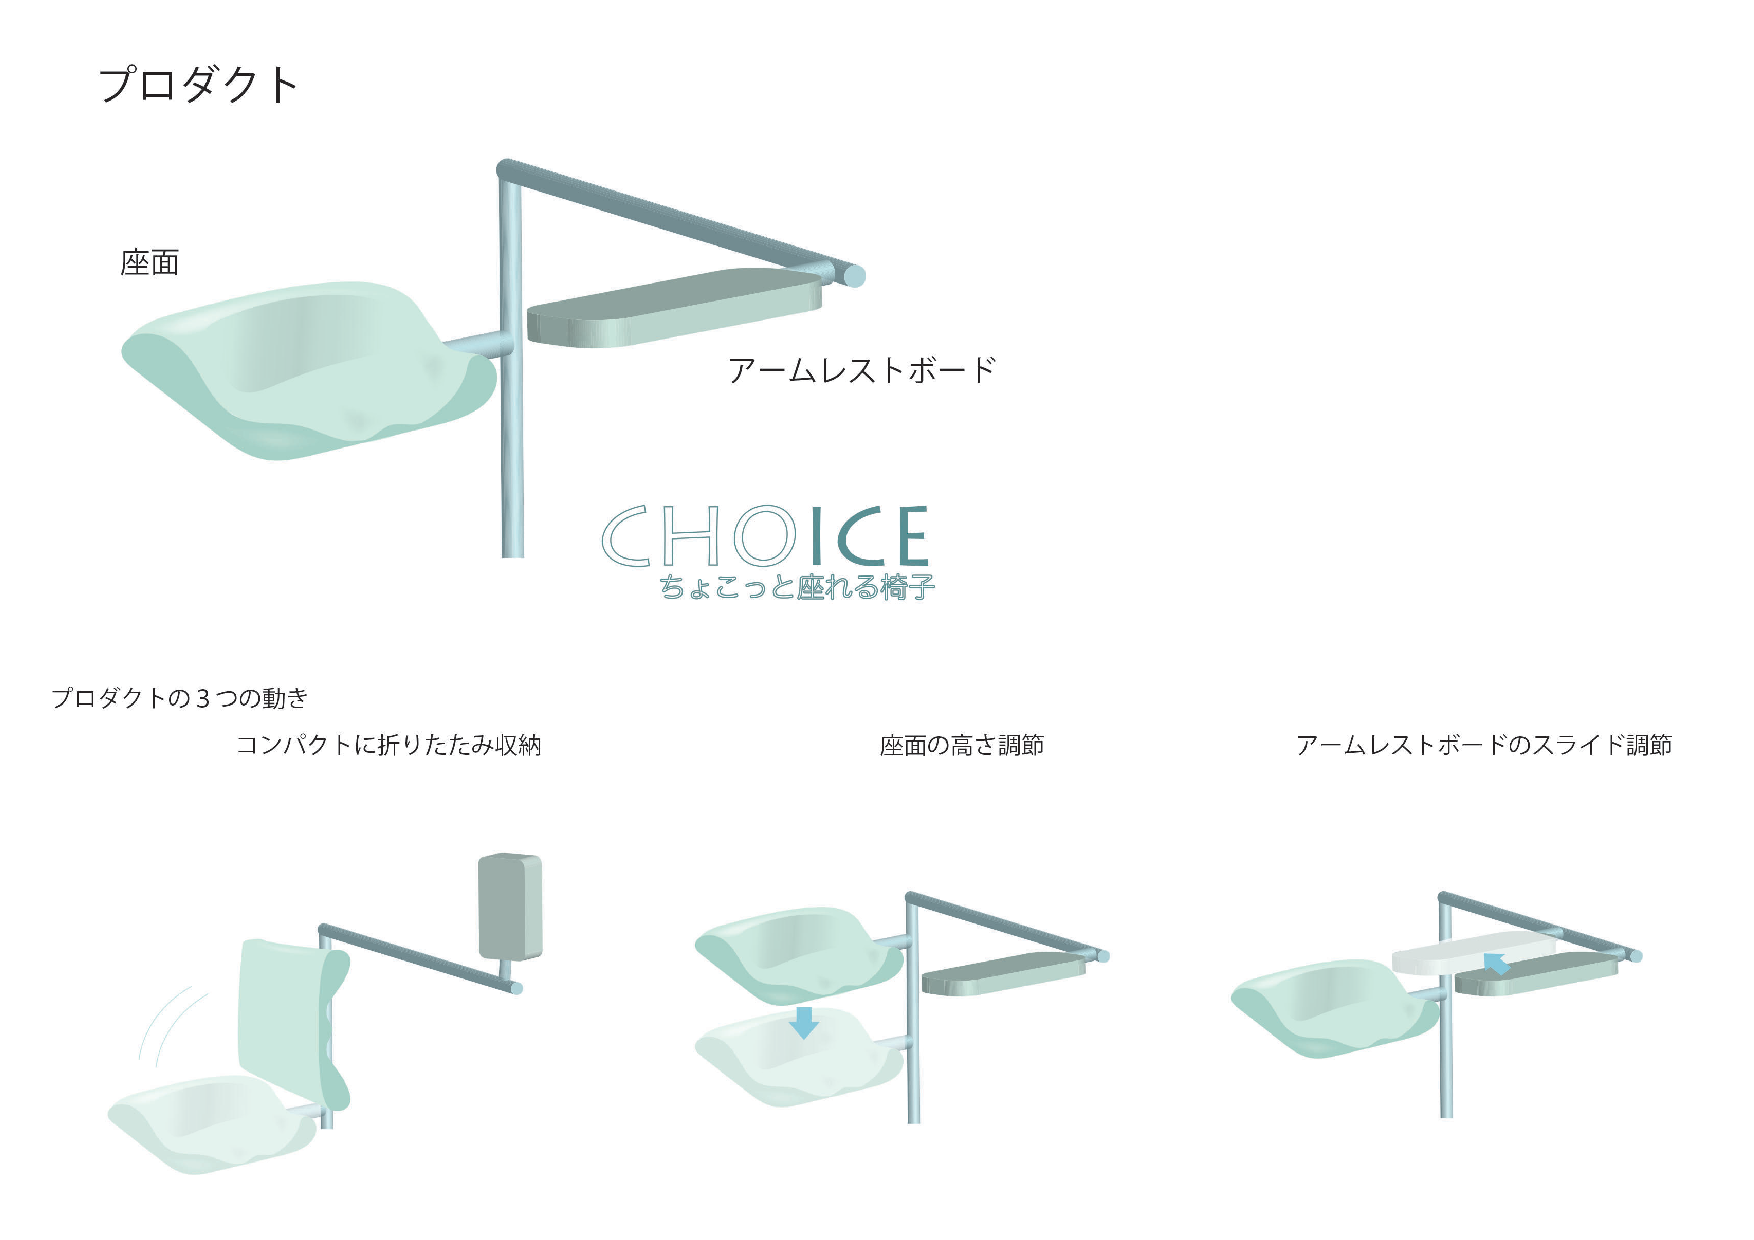
\includegraphics[clip,width=12cm]{images.pdf}
    \caption{開発した製品}
    \label{サンプル図}
  \end{center}
\end{figure}


\section{今後の計画}

今後は,実際に製品の試作品を制作しどのようにしたら使い勝手が良いか.安全性は確実かなどを検証する.改善点が見えたら試作と検証を繰り返す.

プロジェクト終結フェーズへ向けてプロダクトのまとめ等をする.

\bibliographystyle{junsrt}
\bibliography{biblio}%「biblio.bib」というファイルが必要.

\end{document}
